\tikzset{every picture/.style={line width=0.75pt}} %set default line width to 0.75pt        

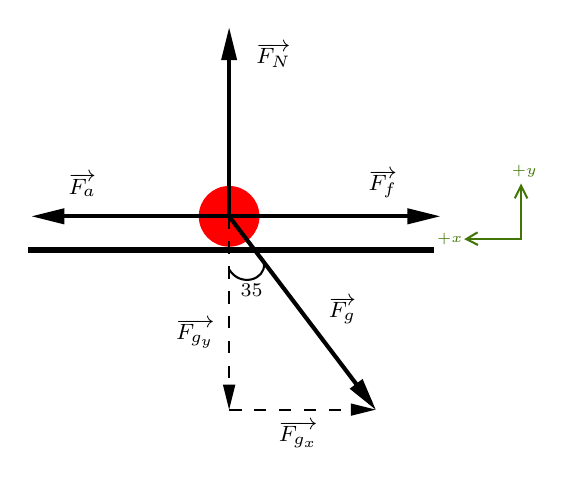
\begin{tikzpicture}[x=0.75pt,y=0.75pt,yscale=-1,xscale=1]
	%uncomment if require: \path (0,300); %set diagram left start at 0, and has height of 300

	%Shape: Ellipse [id:dp6837769595509937] 
	\draw  [color={rgb, 255:red, 255; green, 0; blue, 0 }  ,draw opacity=1 ][fill={rgb, 255:red, 255; green, 0; blue, 0 }  ,fill opacity=1 ] (171.69,144.54) .. controls (171.69,136.74) and (178.01,130.42) .. (185.81,130.42) .. controls (193.61,130.42) and (199.93,136.74) .. (199.93,144.54) .. controls (199.93,152.34) and (193.61,158.66) .. (185.81,158.66) .. controls (178.01,158.66) and (171.69,152.34) .. (171.69,144.54) -- cycle ;
	%Shape: Rectangle [id:dp5669474684894344] 
	\draw  [fill={rgb, 255:red, 0; green, 0; blue, 0 }  ,fill opacity=1 ] (89.25,159.81) -- (283.9,159.81) -- (283.9,161.71) -- (89.25,161.71) -- cycle ;
	%Straight Lines [id:da9589017384386354] 
	\draw [line width=1.5]    (185.81,144.54) -- (185.81,57.7) ;
	\draw [shift={(185.81,53.7)}, rotate = 90] [fill={rgb, 255:red, 0; green, 0; blue, 0 }  ][line width=0.08]  [draw opacity=0] (15.6,-3.9) -- (0,0) -- (15.6,3.9) -- cycle    ;
	%Straight Lines [id:da8525534561361983] 
	\draw [line width=1.5]    (185.81,144.54) -- (283.33,144.54) ;
	\draw [shift={(287.33,144.54)}, rotate = 180] [fill={rgb, 255:red, 0; green, 0; blue, 0 }  ][line width=0.08]  [draw opacity=0] (15.6,-3.9) -- (0,0) -- (15.6,3.9) -- cycle    ;
	%Straight Lines [id:da3080158689414496] 
	\draw [line width=1.5]    (185.81,144.54) -- (94.78,144.54) ;
	\draw [shift={(90.78,144.54)}, rotate = 360] [fill={rgb, 255:red, 0; green, 0; blue, 0 }  ][line width=0.08]  [draw opacity=0] (15.6,-3.9) -- (0,0) -- (15.6,3.9) -- cycle    ;
	%Straight Lines [id:da8911911774184844] 
	\draw [line width=1.5]    (185.81,144.54) -- (254,234.48) ;
	\draw [shift={(256.42,237.67)}, rotate = 232.83] [fill={rgb, 255:red, 0; green, 0; blue, 0 }  ][line width=0.08]  [draw opacity=0] (15.6,-3.9) -- (0,0) -- (15.6,3.9) -- cycle    ;
	%Straight Lines [id:da46681259455801327] 
	\draw  [dash pattern={on 4.5pt off 4.5pt}]  (185.81,144.54) -- (185.81,235.67) ;
	\draw [shift={(185.81,237.67)}, rotate = 270] [fill={rgb, 255:red, 0; green, 0; blue, 0 }  ][line width=0.08]  [draw opacity=0] (12,-3) -- (0,0) -- (12,3) -- cycle    ;
	%Straight Lines [id:da7668757848253749] 
	\draw  [dash pattern={on 4.5pt off 4.5pt}]  (185.81,237.67) -- (254.42,237.67) ;
	\draw [shift={(256.42,237.67)}, rotate = 180] [fill={rgb, 255:red, 0; green, 0; blue, 0 }  ][line width=0.08]  [draw opacity=0] (12,-3) -- (0,0) -- (12,3) -- cycle    ;
	%Shape: Right Angle [id:dp6552113389685195] 
	\draw  [color={rgb, 255:red, 65; green, 117; blue, 5 }  ,draw opacity=1 ] (299.83,155.63) -- (326.43,155.63) -- (326.43,129.75) ;
	%Curve Lines [id:da23057035772319456] 
	\draw    (185.81,170.11) .. controls (191.15,178.89) and (203.37,175.07) .. (202.6,167.44) ;
	\draw  [color={rgb, 255:red, 65; green, 117; blue, 5 }  ,draw opacity=1 ] (323.41,135.88) -- (326.46,129.8) -- (329.5,135.89) ;
	\draw  [color={rgb, 255:red, 65; green, 117; blue, 5 }  ,draw opacity=1 ] (305.7,158.34) -- (300.09,155.5) -- (305.52,152.26) ;

	% Text Node
	\draw (197.44,59.61) node [anchor=north west][inner sep=0.75pt]  [font=\footnotesize] [align=left] {$\displaystyle \overrightarrow{F_{N}}$};
	% Text Node
	\draw (251.55,120.59) node [anchor=north west][inner sep=0.75pt]  [font=\footnotesize] [align=left] {$\displaystyle \overrightarrow{F_{f}}$};
	% Text Node
	\draw (106.94,122.38) node [anchor=north west][inner sep=0.75pt]  [font=\footnotesize] [align=left] {$\displaystyle \overrightarrow{F_{a}}$};
	% Text Node
	\draw (232.34,181.77) node [anchor=north west][inner sep=0.75pt]  [font=\footnotesize] [align=left] {$\displaystyle \overrightarrow{F_{g}}$};
	% Text Node
	\draw (158.72,192.62) node [anchor=north west][inner sep=0.75pt]  [font=\footnotesize] [align=left] {$\displaystyle \overrightarrow{F_{g_{y}}}$};
	% Text Node
	\draw (208.24,241.54) node [anchor=north west][inner sep=0.75pt]  [font=\footnotesize] [align=left] {$\displaystyle \overrightarrow{F_{g_{x}}}$};
	% Text Node
	\draw (189.83,175.58) node [anchor=north west][inner sep=0.75pt]  [font=\scriptsize] [align=left] {$\displaystyle 35\degree $};
	% Text Node
	\draw (284.5,151) node [anchor=north west][inner sep=0.75pt]  [font=\tiny,color={rgb, 255:red, 65; green, 117; blue, 5 }  ,opacity=1 ] [align=left] {$\displaystyle +x$};
	% Text Node
	\draw (320.5,118.5) node [anchor=north west][inner sep=0.75pt]  [font=\tiny,color={rgb, 255:red, 65; green, 117; blue, 5 }  ,opacity=1 ] [align=left] {$\displaystyle +y$};


\end{tikzpicture}